\section{Introduction}\label{sect:introduction}
\new{
Humans have always been trying to monitor the passing of time and to hand down
information for posterity.  The 1989 Oxford English
Dictionary~\cite{dictionary1989oxford} defines a {\em time capsule} as ``{\em a
container used to store for posterity a selection of objects thought to be
representative of life at a particular time}''.  After storing documents and
memories inside the time capsule, they are generally buried underground,
sometimes even sent out to space~\cite{jarvis2015time}.  Time capsules can also
be employed to unconditionally reveal secrets at a future date.

Starting from the 90's, researchers have been designing techniques to create a
digital counterpart of the physical time capsule~\cite{may1993timed} and they
named these techniques {\em Time-Locks}.
}


%Humans have always been trying to monitor the passing of time and to hand down information for posterity.
%The 1989 Oxford English Dictionary~\cite{dictionary1989oxford} defines a {\em time capsule} as ``{\em a container used to store for posterity a selection of objects thought to be representative of life at a particular time}''.
%After storing documents and memories inside the time capsule, they are generally buried underground, sometimes even sent out to space~\cite{jarvis2015time}.
%Time capsules can also be employed to unconditionally reveal secrets at a future date.

%Starting from the 90's, researchers have been designing techniques to create a digital counterpart of the physical time capsule~\cite{may1993timed}.

A \textit{Time-Lock} (TL) is a primitive that implements the following scheme:
a data owner entrusts a notary with a secret to be disclosed at a
future time; the notary keeps the secret private until then; and finally, the notary discloses it publicly. Once the notary has been entrusted with the secret, the owner is no longer needed for disclosure to happen.
Such primitive can be used in many real-world scenarios, such as voting, inheritance management, and delegated challenge-response protocols.

Notaries~\cite{10.1007/BFb0032349}~\cite{rabin2006time} are not
suitable for all the scenarios~\cite{Abelson:1997:RKR:275079.275104},
as they require the owner to completely entrust a single third party.
Therefore, cryptographers have been designing encryption techniques, known as Time-Lock Encryption (TLE)~\cite{may1993timed}, that enable the deployment of Time-Lock {\em Puzzles}~\cite{mahmoody-tl,Bitansky:2016:TPR:2840728.2840745}.
In the TLE setting, the sending party (i.e., the owner) can encrypt a secret so that the receiving party is required to perform multiple decryptions to recover the secret.
The number of times the decryption algorithm has to be run can be tuned by the sending party during the encryption process.
As long as the time to run the decryption algorithm can be considered approximately constant, it is possible to protect a secret for arbitrarily long periods of time.
In other terms, TLE can be used to create Time-Locks.
Yet, it is worth noting that the disclosure time is not fixed, but it depends on when the decryption process starts.
% and on the amount of computational resources dedicated to the task.

The first TLE scheme was proposed by Rivest, Shamir, and Wagner~\cite{Rivest:1996:TPT:888615}.
The scheme relies on a trapdoor function so that the receiver has to undergo a computing effort that is orders of magnitude greater compared to the one of the sending party. Their approach also imposed the decryption algorithm to be executed in inherently sequential order.
Such kinds of techniques are also known with the name {\em Proof of Sequential Work} ({\em PoSW})~\cite{posw,cohen2018}.

An alternative to the use of trapdoor functions is the use of {\em weak hash-chains}~\cite{gwern}, specifically, it requires the receiver to brute-force a chain of weak hashes to obtain the secret.
The reason a chain is used in place of a single stronger hash is that it permits to reduce the variance associated with the time of the decryption process. 
However, in this setting the decryption process can be parallelized, thus the estimated disclosure time is far less reliable.
These approaches are often associated with {\em Proof of Work (PoW)}~\cite{pow} algorithms.

Yet, two aspects of TLE make them impractical. First,
%Current research efforts mostly rely on Proof-of-Work puzzles that provide guarantees about the time taken by the decryption process.
%These solutions, however, are not practical.
%
the owner has to make assumptions on future computing power. 
This is far from trivial.
As an example, Rivest's LCS35 time-lock puzzle~\cite{lcs35}, whose decryption time was estimated to be 35 years, was cracked in 2019 in just 2 months using dedicated hardware~\cite{lcs35-crack-open}.
 %
%the breakdown in CPU clock-speed and the advent of quantum computing are two examples of hitches in this process\footnote{As a matter of fact, Rivest used his scheme to build a time capsule in 1999. Being his computing power estimate based on the Moore's law, which is not valid anymore, his original estimated time of 35 years to solve the puzzle appears way too optimistic now.}.
%
Secondly, TLE schemes require the receiving party to run the decryption procedure continuously for a long time, which poses a question about incentives.


\medskip\textbf{Our approach.} In this chapter, we present a practical Time-Lock protocol named {\em \name} ({\em \shortname}), based neither on trust assumptions nor on cryptographic puzzles.

The basic idea of our approach is to first split a secret into shares using {\em threshold cryptography} (i.e., Shamir's Secret Sharing~\cite{Shamir:1979:SS:359168.359176}), and assign them to users so that no one can recover the secret unless \KofN shares are available.
To ensure the TL behavior, we rely on economic incentives and penalties enforced by a smart contract.
The contract rewards users for revealing their share only after the disclosure time and penalizes any other misbehavior.
% (i.e., the disclosure of it). 
Rational users will always comply with the protocol, as we constraint that only correctly behaving is economically convenient, thus effectively deploying a distributed time-lock mechanism.

As rewards and penalties are associated with the correct management of the shares, it is important to confidentially generate and distribute them, even in the presence of a dishonest secret's owner.
In our prototype, we address this by using {\em secure Multi-Party Computation (sMPC)}.
% to have guarantees about the information that every participant gets to know.
%
We show a comparison between \shortname  and other Time-Lock techniques in Figure~\ref{fig:models}.
% compares \shortname with the existing Time-Lock techniques.

\begin{figure}[t]
	\centering
	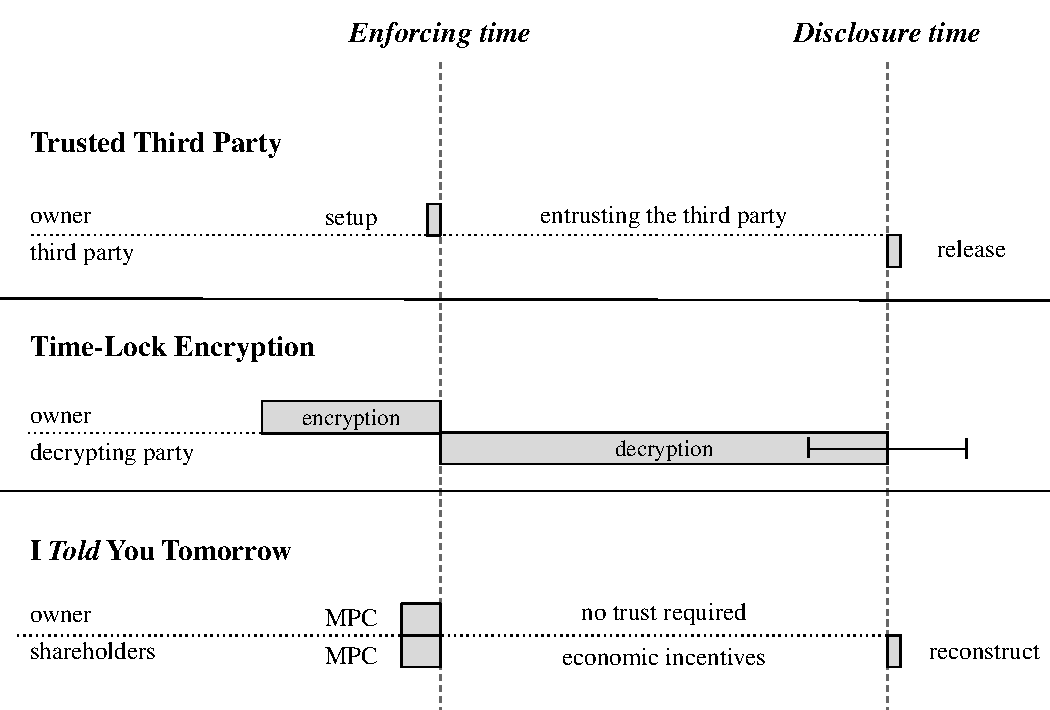
\includegraphics[width=1.0\textwidth]{fig/models}
	\caption{Activities comparison for subjects involved in different TL approaches}
	\label{fig:models}
\end{figure}


\begin{itemize}
	\item Trusted Third Party benefits from a short setup time but relies on a strong trust assumption.
	
	\item Time-Lock Encryption does not depend on trust assumptions, but it requires the receiving party to continuously execute the decryption routine from enforcing till disclosure time.
	
	\item {\em \name} allows the owner of a secret to practically disclose it at a future point in time without requiring her to take part in the disclosure protocol. It relies only on economic incentives.
\end{itemize}

\noindent The main contributions of this chapter can be summarized as follows.\todo{fix contributions, This looks more ``what we did'' rather than our contributions}

\begin{enumerate}

	\smallskip
 	\item We define a practical and abstract method to deploy Time-Locked secrets on the blockchain by leveraging an economic model in which every actor (or coalition of them) has an expected negative payoff associated with any possible misbehavior.
 	
 	\smallskip
 	\item We address the problems that arise when combining secure Multi-Party Computation and protocols based on economic incentives and penalties. 
  
  	\smallskip
 	\item We describe how to technically realize an implementation based on the Ethereum blockchain~\cite{wood2014ethereum} and the FRESCO secure Multi-Party Computation framework~\cite{damgaard2016mpc}, characterized by low overhead and limited gas cost of execution.

\end{enumerate}


